
Über die Navigationsleiste auf der linken Seite kann der Benutzer die Einstellungen aufrufen. In diesem Bereich lassen sich verschiedene Verhaltensweisen der Anwendung anpassen.

\begin{itemize}
    \item \textbf{Dateien direkt löschen:} Wenn diese Option aktiviert ist, werden erkannte Dateien unmittelbar entfernt. Ist sie deaktiviert, landen die Dateien zunächst im Papierkorb, was eine Wiederherstellung ermöglicht.
    \item \textbf{Rekursiv löschen:} Diese Option bestimmt, ob auch Unterordner des angegebenen Verzeichnisses durchsucht und bereinigt werden sollen.
\end{itemize}

Zusätzlich besteht die Möglichkeit, das Benutzerpasswort zu ändern. Dazu muss zunächst das aktuelle Passwort eingegeben werden, gefolgt von der Eingabe und Bestätigung eines neuen Passworts. Das System prüft, ob das neue Passwort den Sicherheitsrichtlinien entspricht und ob beide Eingaben übereinstimmen.

\begin{figure}[H]
    \centering
    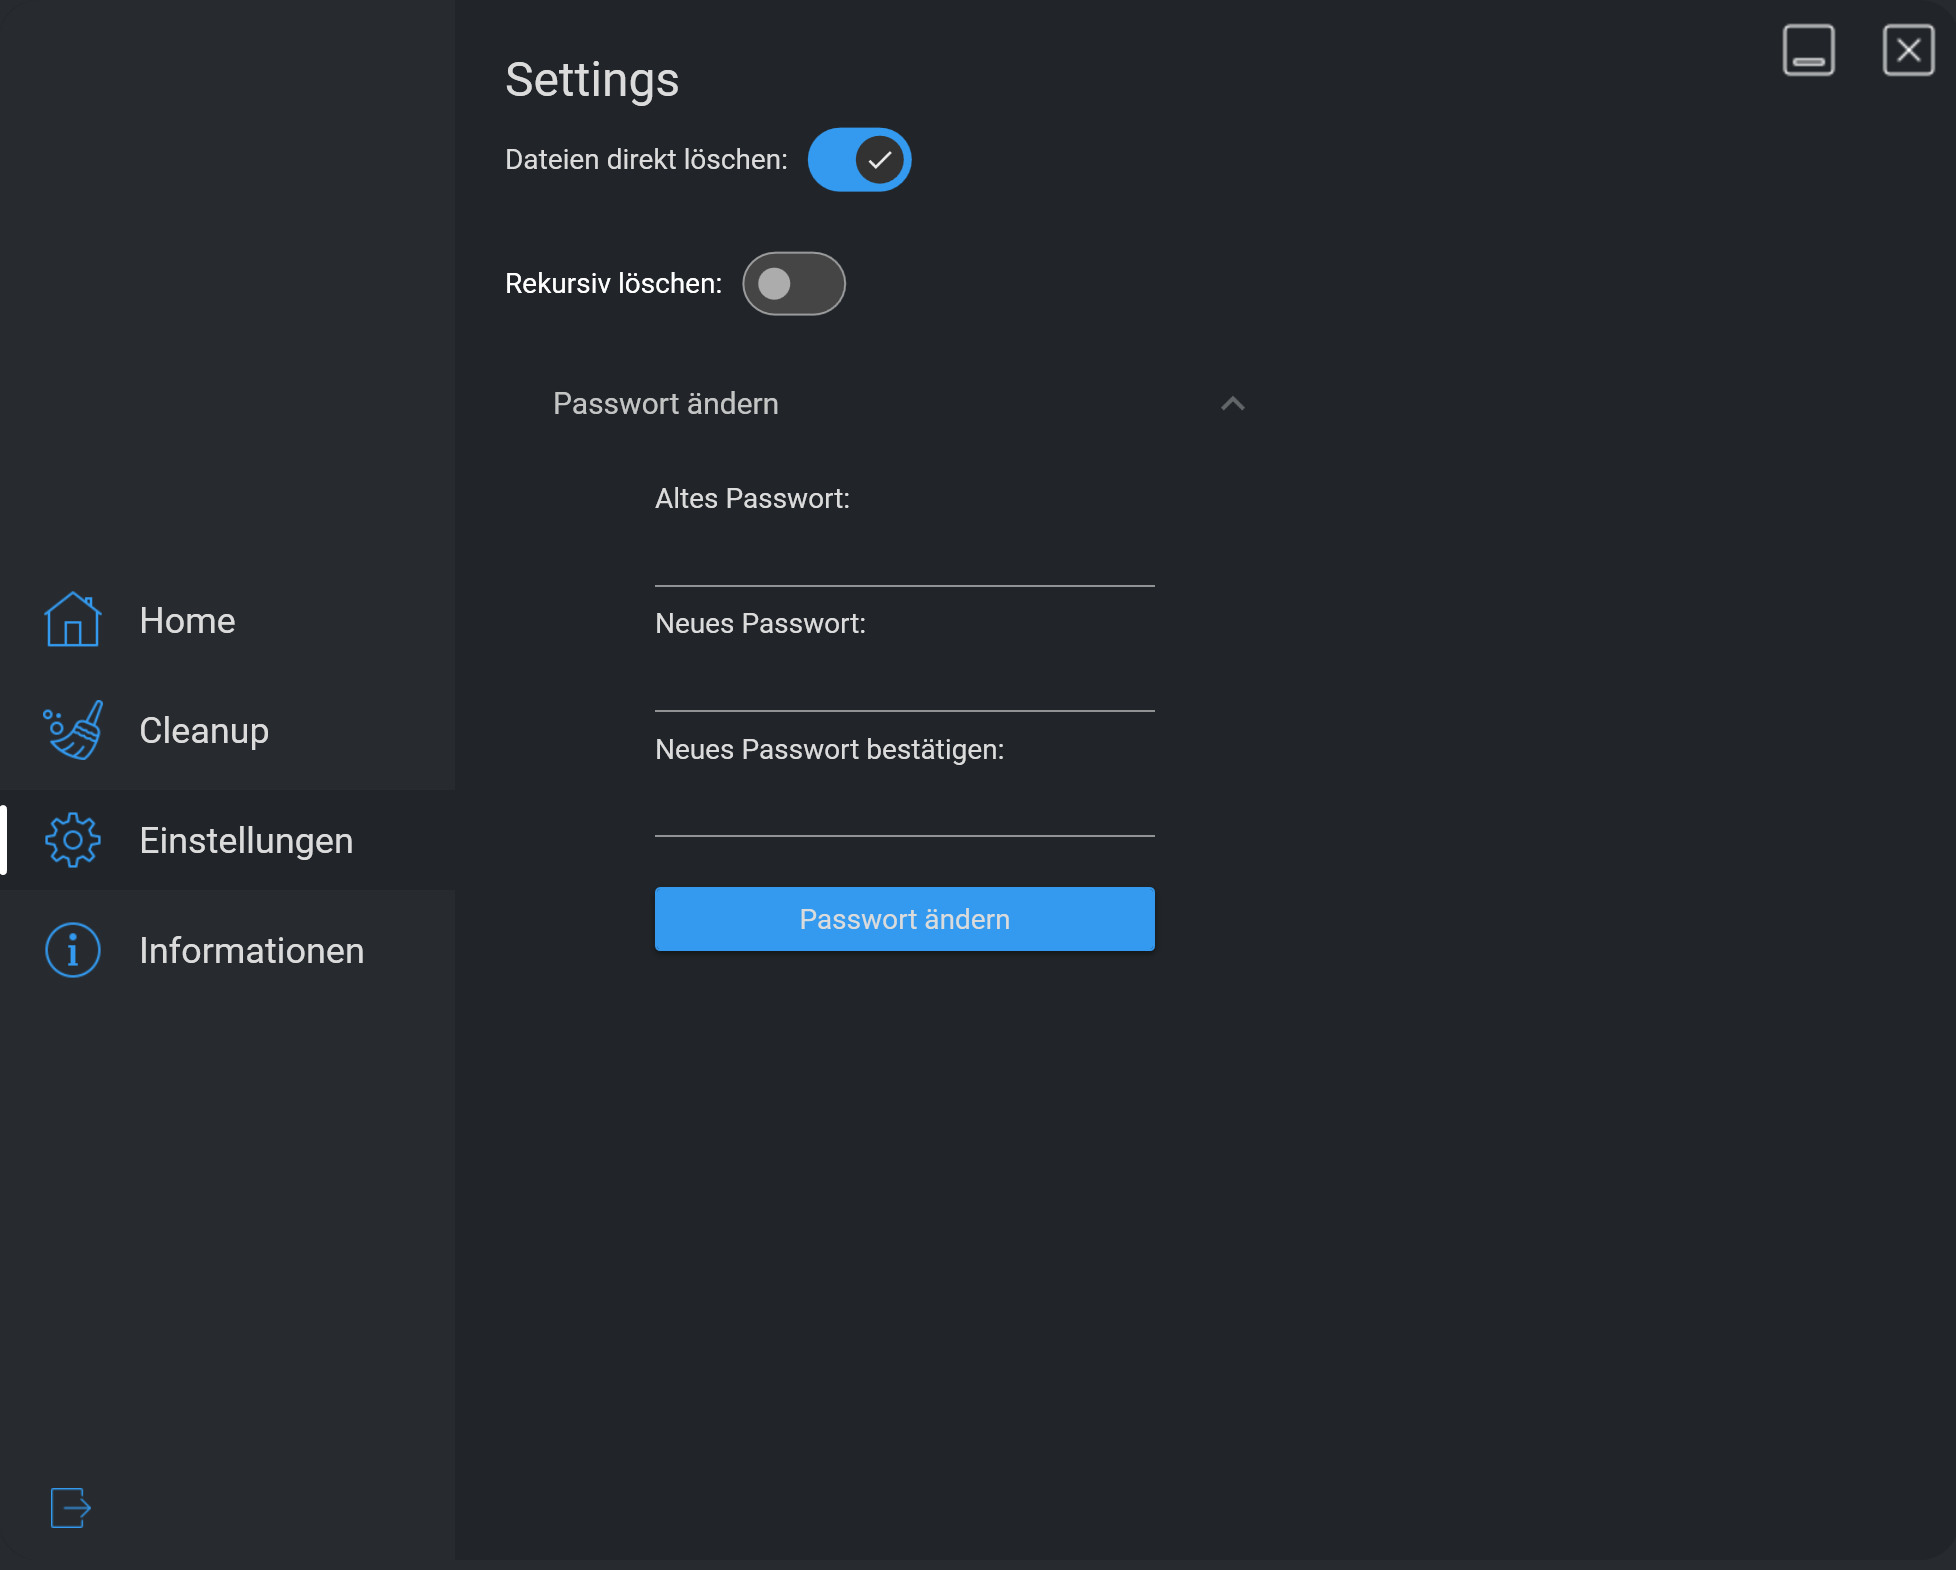
\includegraphics[width=0.9\textwidth]{src/screenshot_settings.png}
    \caption{Einstellungsseite mit Optionen zur Konfiguration und Passwortänderung}
\end{figure}
